\label{sec:part_1_result_analysis}

Having identified many inconsistencies and ambiguities in the original paper so far, we shall conduct the complete pipeline to reproduce their results.
While working on this, we are aware of another critical inconsistency in their reported results, in some parts, they mention the use of 10–fold cross validation (CV), e.g. the tables presenting the per–class performance metrics of their models.
Meanwhile, no explanation on the use of 10–fold CV nor single train/test split for the confusion matrices.

In \textbf{Sec. \ref{sec:part_1_method}}, we introduce the methodologies and protocols in our pipeline as an attempt to reproduce the results presented in \cite{sinha2023dasmcc}.
Nonetheless, they are quite fragmented, and thus, we shall unify them into one single pipeline as below.

\begin{figure}[H]
\centering
\begin{tikzpicture}[
    font=\footnotesize,
    stage/.style = {draw, rounded corners=2pt, align=center, inner sep=3pt,
                    minimum height=9mm, text width=26mm},
    com/.style   = {stage, fill=black!6},
    lane/.style  = {stage, text width=38mm, fill=black!2},
    head/.style  = {stage, text width=38mm, fill=black!12, font=\footnotesize\bfseries},
    fork/.style  = {stage, text width=34mm, fill=black!12, font=\footnotesize\bfseries},
    arr/.style   = {-{Stealth[length=2mm]}, semithick}
]
% ---------- common stages ----------
\node[com] (s1) at (0,0)     {\textbf{1.} Preprocessing\\ $(1000\times 12)\to(12000,)$};
\node[com] (s2) at (3.3,0)   {\textbf{2.} Feature extraction\\ \texttt{neurokit2}: $\to(16,N)$};
\node[com] (s3) at (6.6,0)   {\textbf{3.} Impute \& align\\ \texttt{ffill}, $N$ = R–peak median\\ $\to 16 \times N$ features};
\node[com] (s4) at (9.9,0)   {\textbf{4.} Label encoding\\ NORM$\dots$CD $\to 0\dots4$};
\draw[arr] (s1) -- (s2);
\draw[arr] (s2) -- (s3);
\draw[arr] (s3) -- (s4);

% ---------- fork ----------
\node[fork] (s5) at (4.95,-1.9) {5. Partitioning};
\draw[arr] (s4.south) -- ++(0,-0.45) -| (s5.north);

% ---------- protocol A ----------
\node[head] (a1) at (2.1,-3.5) {Protocol A\\ single $80/20$ split};
\node[lane] (a2) at (2.1,-5.0) {Scale $+$ \texttt{SMOTE}\\ on train split only};
\node[lane] (a3) at (2.1,-6.4) {Fit the 6 classifiers};
\node[lane] (a4) at (2.1,-7.8) {Evaluate on test split\\ \emph{(confusion matrices, class–wise ROC curves)}};
\draw[arr] (a1) -- (a2); \draw[arr] (a2) -- (a3); \draw[arr] (a3) -- (a4);

% ---------- protocol B ----------
\node[head] (b1) at (7.8,-3.5) {Protocol B\\ $10$--fold CV};
\node[lane] (b2) at (7.8,-5.0) {Scale $+$ \texttt{SMOTE}\\ on the 9 training folds};
\node[lane] (b3) at (7.8,-6.4) {Fit the 6 classifiers};
\node[lane] (b4) at (7.8,-7.8) {Evaluate on held--out fold};
\node[lane] (b5) at (7.8,-9.4) {Average over the $10$ folds\\ \emph{(per–class metrics, across–class metrics)}};
\draw[arr] (b1) -- (b2); \draw[arr] (b2) -- (b3); \draw[arr] (b3) -- (b4);
\draw[arr] (b4) -- (b5);

% repeat bracket
\draw[dashed, black!55, rounded corners=3pt]
     ($(b2.north west)+(-0.35,0.18)$) rectangle ($(b4.south east)+(0.35,-0.18)$);
\node[font=\scriptsize\itshape, black!55, anchor=west]
     at ($(b2.north east)+(0.42,0.05)$) {$\times\,10$};

% ---------- fork arrows ----------
\draw[arr] (s5.south) -- ++(0,-0.4) -| (a1.north);
\draw[arr] (s5.south) -- ++(0,-0.4) -| (b1.north);
\end{tikzpicture}
\caption{Unified reproduction pipeline.}
\label{fig:pipeline}
\end{figure}

\subsection{Reproduced versus Published Results}

We use \texttt{HistGradientBoostingClassifier} as alternative to \texttt{GradientBoostingClassifier} due to computing resources constraints, and their provably near–similar performance.

\begin{table}[H]
    \centering
    \caption{\textbf{Protocol B} class–wise performance metrics across models.}
    \label{tab:cv_classwise}

    \begin{subtable}[t]{0.48\textwidth}
        \centering
        \caption{KNN}
        \label{tab:cv_knn}
        \begin{tabular}{cccc}
            \toprule
            Class & Precision & Recall & F1 Score \\
            \midrule
            NORM (0) & 64.7	& 23.7 & 34.7 \\
            MI   (1) & 19.8 & 35.6 & 25.4 \\
            STTC (2) & 18.5	& 29.3 &	22.7 \\
            HYP  (3) & 16.7 & 34.9 &	22.5 \\
            CD   (4) & 16.3	& 32.8 & 21.7 \\
            \bottomrule
        \end{tabular}
    \end{subtable}
    \hfill
    \begin{subtable}[t]{0.48\textwidth}
        \centering
        \caption{Random Forest}
        \label{tab:cv_rf}
        \begin{tabular}{cccc}
            \toprule
            Class & Precision & Recall & F1 Score \\
            \midrule
            NORM (0) & 66.0 & 76.1 & 70.7 \\
            MI   (1) & 37.0 & 27.7 & 31.7 \\
            STTC (2) & 29.6 & 23.9 & 26.4 \\
            HYP  (3) & 30.4 & 40.7 & 34.6 \\
            CD   (4) & 39.1 & 27.9 & 32.5 \\
            \bottomrule
        \end{tabular}
    \end{subtable}

    \bigskip

    \begin{subtable}[t]{0.48\textwidth}
        \centering
        \caption{Histogram–based Gradient Boosting}
        \label{tab:cv_gb}
        \begin{tabular}{cccc}
            \toprule
            Class & Precision & Recall & F1 Score \\
            \midrule
            NORM (0) & 65.1 & 87.6 & 74.7 \\
            MI   (1) & 45.9 & 26.1 & 33.2 \\
            STTC (2) & 35.7 & 16.8 & 22.7 \\
            HYP  (3) & 40.8 & 32.3 & 35.8 \\
            CD   (4) & 48.0 & 28.9 & 36.0 \\
            \bottomrule
        \end{tabular}
    \end{subtable}
    \hfill
    \begin{subtable}[t]{0.48\textwidth}
        \centering
        \caption{AdaBoost}
        \label{tab:cv_ada}
        \begin{tabular}{cccc}
            \toprule
            Class & Precision & Recall & F1 Score \\
            \midrule
            NORM (0) & 67.4 & 39.8 & 49.9 \\
            MI   (1) & 21.6 & 27.2 & 23.9 \\
            STTC (2) & 22.0 & 29.8 & 25.2 \\
            HYP  (3) & 14.8 & 62.9 & 23.9 \\
            CD   (4) & 20.3 & 25.1 & 22.3 \\
            \bottomrule
        \end{tabular}
    \end{subtable}

    \bigskip

    \begin{subtable}[t]{0.48\textwidth}
        \centering
        \caption{CatBoost}
        \label{tab:cv_cat}
        \begin{tabular}{cccc}
            \toprule
            Class & Precision & Recall & F1 Score \\
            \midrule
            NORM (0) & 66.0 & 85.0 & 74.3 \\
            MI   (1) & 44.4 & 31.0 & 36.5 \\
            STTC (2) & 35.1 & 19.0 & 24.5 \\
            HYP  (3) & 35.9 & 29.7 & 32.1 \\
            CD   (4) & 46.3 & 28.3 & 35.0 \\
            \bottomrule
        \end{tabular}
    \end{subtable}
    \hfill
    \begin{subtable}[t]{0.48\textwidth}
        \centering
        \caption{XGBoost}
        \label{tab:cv_xgb}
        \begin{tabular}{cccc}
            \toprule
            Class & Precision & Recall & F1 Score \\
            \midrule
            NORM (0) & 65.0 & 86.9 & 74.3 \\
            MI   (1) & 45.4 & 28.1 & 34.7 \\
            STTC (2) & 34.5 & 16.8 & 22.4 \\
            HYP  (3) & 40.8 & 26.6 & 32.0 \\
            CD   (4) & 45.0 & 26.6 & 33.4 \\
            \bottomrule
        \end{tabular}
    \end{subtable}
\end{table}

We present the table below to compare with their Table 12, and we complement it with a wall–clock time column, for sake of comparison against our proposed solution in \href{sec:part_2}{Part 2}.
More precisely, the time reported throughout this report refers to the time taken by the classifiers in \textbf{Protocol B}, i.e. 10–fold CV - including both training and testing, said differently, the actual inference speed is much shorter than that, and we omit the time taken by feature extractors.

\begin{table}[H]
    \centering
    \caption{\textbf{Protocol B} Performance metrics across all models.}
    \label{tab:single_model_wise}
    \begin{tabular}{ccccccc}
        \toprule
        Metrics & \texttt{XGBoost} & \texttt{RF} & \texttt{CatBoost} & \texttt{AdaBoost} & \texttt{GBoost} & \texttt{KNN} \\
        \midrule
        Precision & 46.1 & 40.4 & 45.5 & 29.2 & 47.1 & 27.2 \\
        Recall & 37.0 & 39.3 & 38.6 & 37.0 & 38.3 & 31.2 \\
        F1 Score & 39.4 & 39.2 & 40.5 & 29.0 & 40.5 & 25.4 \\
        Accuracy & 59.0 & 54.6 & 59.0 & 35.6 & 59.6 & 27.7 \\
        \midrule
        \midrule
        Time (s) & 49.5 & 57.2 & 282.7 & 322.2 & 140.7 & 2.3 \\
        \bottomrule
    \end{tabular}
\end{table}

\begin{figure}[H]
    \centering
    \caption{\textbf{Protocol A} Confusion matrices of all classifiers.}
    \label{fig:reproduced_confusion}
    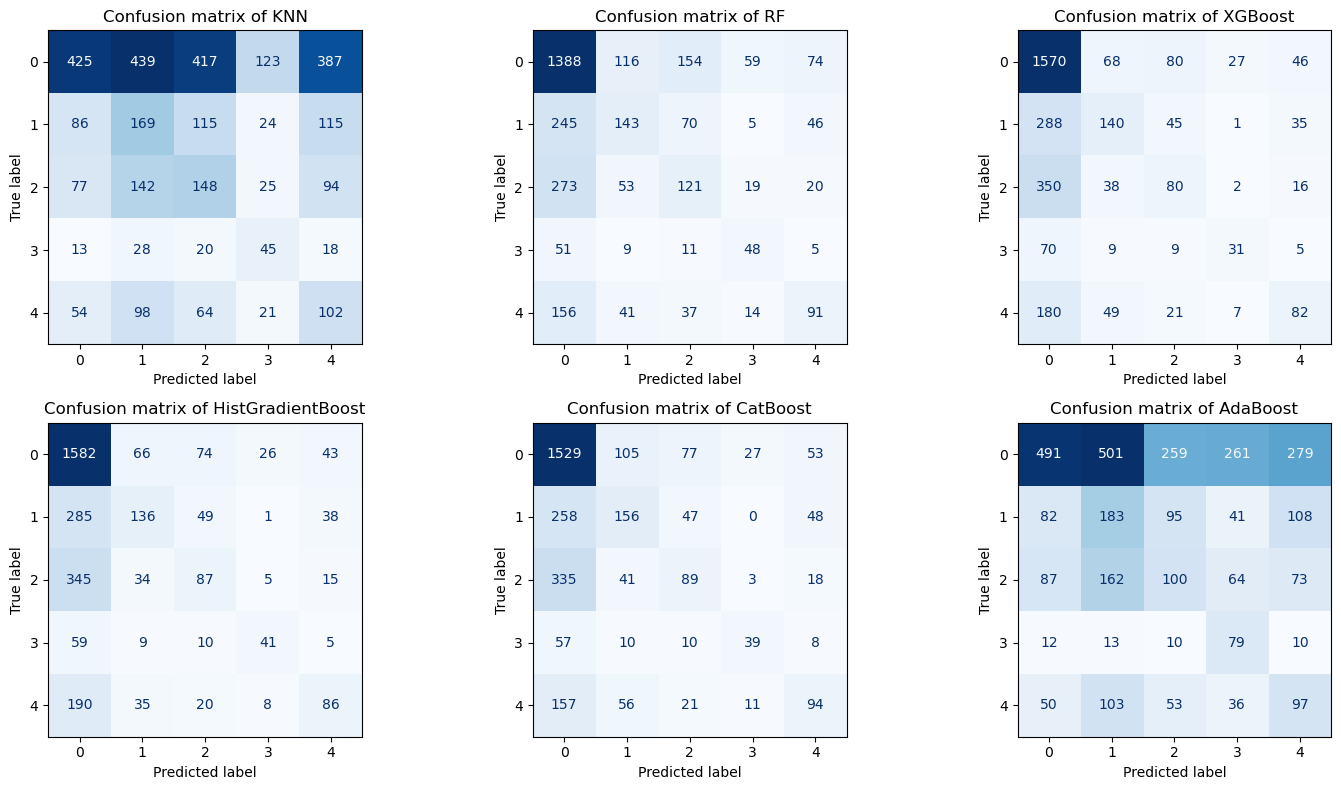
\includegraphics[width=\textwidth]{figures/part1/reproduced_confusion.png}
\end{figure}

\begin{figure}[H]
    \centering
    \caption{\textbf{Protocol A} ROC–AUC curves and scores across classifiers.}
    \label{fig:reproduced_roc}
    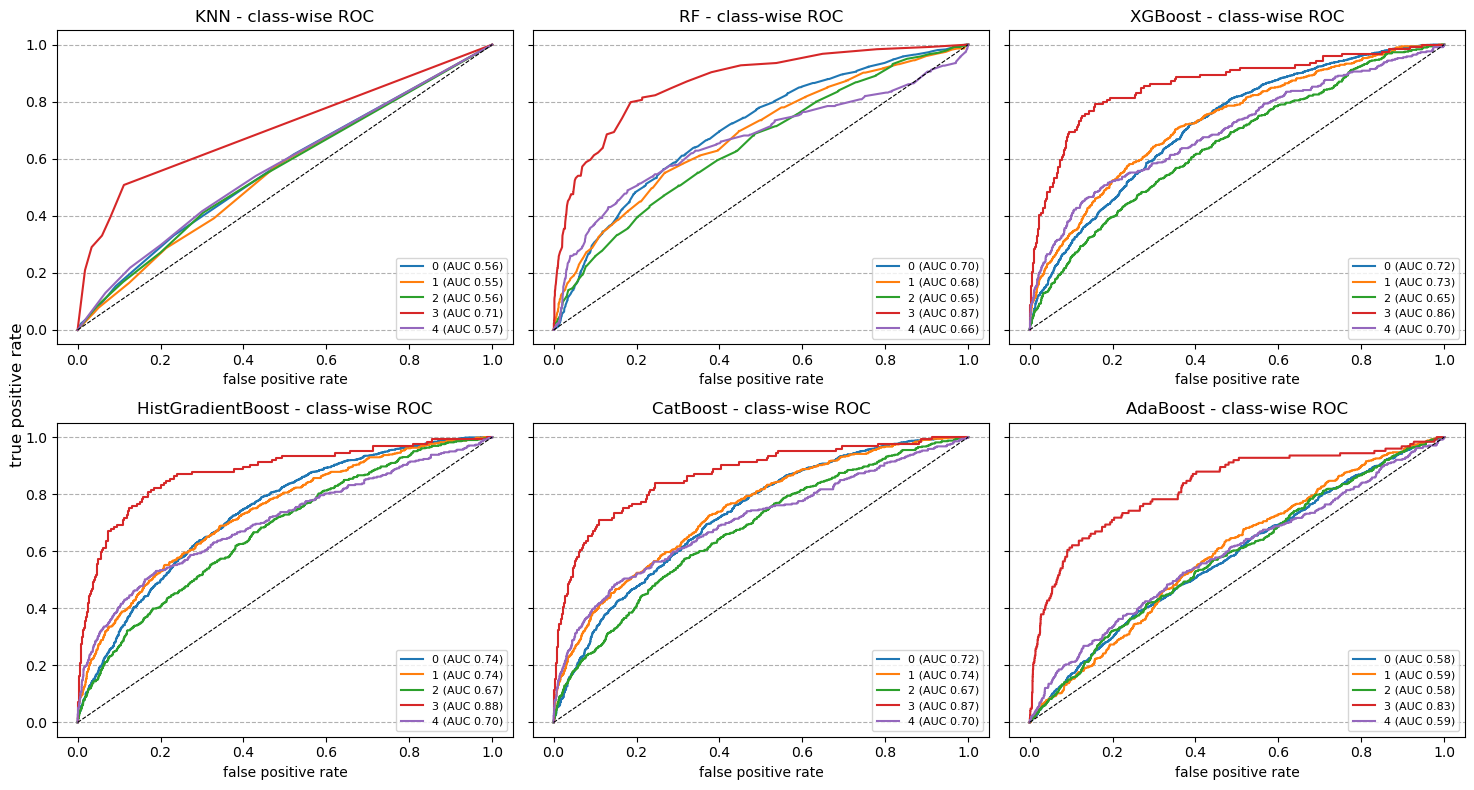
\includegraphics[width=\textwidth]{figures/part1/reproduced_roc_curve.png}
\end{figure}

\subsection{Critical Analysis of Discrepancies}
\label{sec:part_1_discrepancy}

From the outputs above, we are unable to reproduce the results presented in the original paper.

In particular, their Table 12 places XGBoost first at $93.0$ F1 and $93.0\%$ accuracy, followed by RF ($92.0$, $91.0\%$), CatBoost ($89.0$, $89.0\%$), G–Boost ($87.0$, $88.0\%$) and KNN ($83.0$, $82.0\%$). 
The corresponding entries of \textbf{Tab. \ref{tab:single_model_wise}} are $39.4$, $39.2$, $40.5$, $40.5$ and $25.4$ F1, witnessing significant drops between $46$ and $58$. 
Noticeably, in their Tables 6, 7, 9, 10 and 11, HYP is the easiest class for every model, at F1 $96$–$99$, whereas NORM is the hardest, at $56$–$86$. 
In our \textbf{Tab. \ref{tab:cv_classwise}}, NORM is our strongest class throughout, at $34.7$–$74.7$, and the three minority classes collapse to $21.7$–$36.0$.

The \textbf{Fig. \ref{fig:reproduced_confusion}} is evaluated on held–out records, i.e. a single 80/20 train/test split. Therefore, the confusion matrices showcasing all models perform best for the most prevalent class in \texttt{PTB–XL}, i.e. NORM, and the models misclassify the other classes, mostly as the prevalent class.
Meanwhile, their Figure 7, the distribution of classes are almost equivalent. More thorough quantitative observation is set out below.

Looking at the ROC curves for \texttt{XGBoost}, their Figure 8 reports class–wise AUC from 0.98 to 1.00, whereas our \textbf{Fig. \ref{fig:reproduced_roc}} reports from 0.70 to 0.86, significantly diverge from their results.
Although we agree with them that HYP is most easily separable class, their models, especially \texttt{KNN} captures all HYP classes in the test set is a clear signal of interpolation.
In other words, the distribution of HYP in both train and test sets should be very similar, so that \texttt{KNN} can capture all of them, and thus, highly likely data leakage is presented, owing to \texttt{SMOTE} before train/test split.

Regarding the the extra model \texttt{AdaBoost}, our \texttt{CatBoost} attains $40.5$ F1 at $59.0\%$ accuracy against \texttt{AdaBoost}'s $29.0$ and $35.6\%$, implying that, they indeed made a typo error in their abstract section.

We shall present some basic calculations based on their figures, and claim the inconsistencies throughout their paper herein.

Looking at their ``Table 3. Distribution of diagnostic superclasses'', we have:
\begin{itemize}
     \item \texttt{SMOTE} after train/test split
          \begin{itemize}
               \item Total sampples: $9528 + 4907 + 5250 + 2655 + 5486 = 27826$
               \item 80\% train: $27826 \times 80\% \approx 22261$
               \item 20\% test: $27826 \times 20\% \approx 5565$
          \end{itemize}
     \item \texttt{SMOTE} before train/test split
          \begin{itemize}
               \item Total sampples: $9528 \times 5 = 47640$
               \item 80\% train: $47640 \times 80\% = 38112$
               \item 20\% test: $47640 \times 20\% = 9528$
          \end{itemize}
\end{itemize}
Next, let us count the total samples in the test set, by taking into account their confusion matrices presented in their \textbf{Figure 7}. Since all matrices share the same number of test samples, consider ``Confusion Matrix\_KNN'':
$
414 + 547 + 544 + 118 + 231 + 28 + 1748 + 19 + 4 + 10 + 22 + 57 + 1694 + 4 + 10 + 1796 + 15 + 22 + 28 + 6 + 1766 = 9083
$.
As described in their section \textbf{III.E. Data Augmentation}, they stated ``the process of data augmentation and feature scaling is done only on 80\% of training data...''.
We can exclude the possibility that $5565$ is upsampled to $9083$ test samples counted above.
Therefore, it is more likely that they do \texttt{SMOTE} before train/test split.
We also note here, another annotation errors, they name the subcaption (b) and (c) as ``CM of RF'', while the subfigure (c) is ``Confusion Matrix\_XG''

Another apparent evidence is that, by taking the sum across the rows in the ``Confusion Matrix\_KNN'', we have:
\begin{itemize}
     \item NORM (0): $414 + 547 + 544 + 118 + 231 = 1854$
     \item MI (1): $28 + 1748 + 19 + 4 + 10 = 1809$
     \item STTC (2): $22 + 57 + 1694 + 4 + 10 = 1787$
     \item HYP (3): $0 + 0 + 0 + 1796 + 0 = 1796$
     \item CD (4): $15 + 22 + 28 + 6 + 1766 = 1837$
\end{itemize}
The number of samples with respect to each class are almost identical, this is very unlikely to happen if they split the dataset prior to \texttt{SMOTE}, and thus, strongly supporting our point that they leak data into the training.
Meanwhile, in their section \textbf{IV. Result and Discussion}, they stated ``The Confusion Matrices for all the five classifiers with 20\% of testing data are given in Figure 7.'', and indeed, the number of samples HYP (3), according to their Table 3, is 2655.
There exists an extremely tiny probability for one to obtain 1796 test samples in HYP (3) for a 80/20 train/test split.

To reinforce our statements, we shall perform the following ablation study, conducting SMOTE before train/test split and some additional modifications to close the gap between their presented results and reproduced results.
More importantly, the act of \texttt{SMOTE} prior to train/test split, is a kind of data leakage. We present the section below to argue their results, and in fact, the ablation studies below are the closest to their presented results.

\subsection{Ablation study}
\label{sec:ablation_part1}

We shall do the following, details can be found in \texttt{ablation.ipynb}.
In brief, we perform \texttt{StandardScaler()} and \texttt{SMOTE} prior to the train/test split stage, as this would introduce data leakage to the train set, and in fact, significantly improve the results on the test set, though it falsely report models' performance.
We also realise that, either $(1000 \times 12)$ or $(12 \times 1000)$ can be flattened to $(12000,)$, the latter sounds more reasonable, as it places the lead axis before the time axis, and we hypothesize it would describe the raw ECG signals, more meaningfully and precisely.
However, we still keep the same established flattening order, i.e. $(1000 \times 12) \to (12000,)$.
Let us present the results obtained, by keeping the same configuration discussed earlier.

\begin{figure}[H]
    \caption{Comparison on class–wise precision for each model.}
    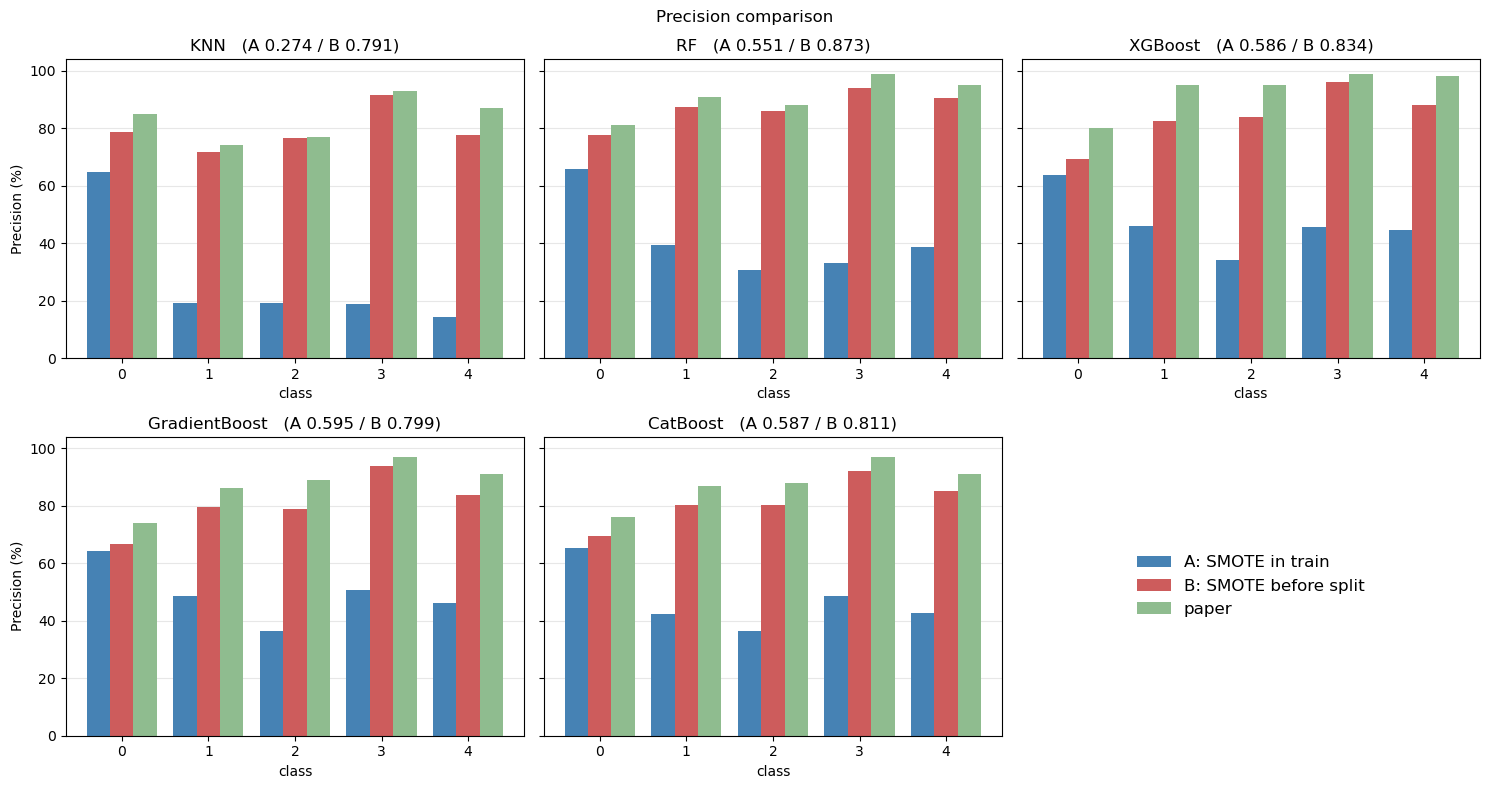
\includegraphics[width=0.9\textwidth]{figures/part1/ablation_precision.png}
\end{figure}

\begin{figure}[H]
    \caption{Comparison on class–wise recall for each model.}
    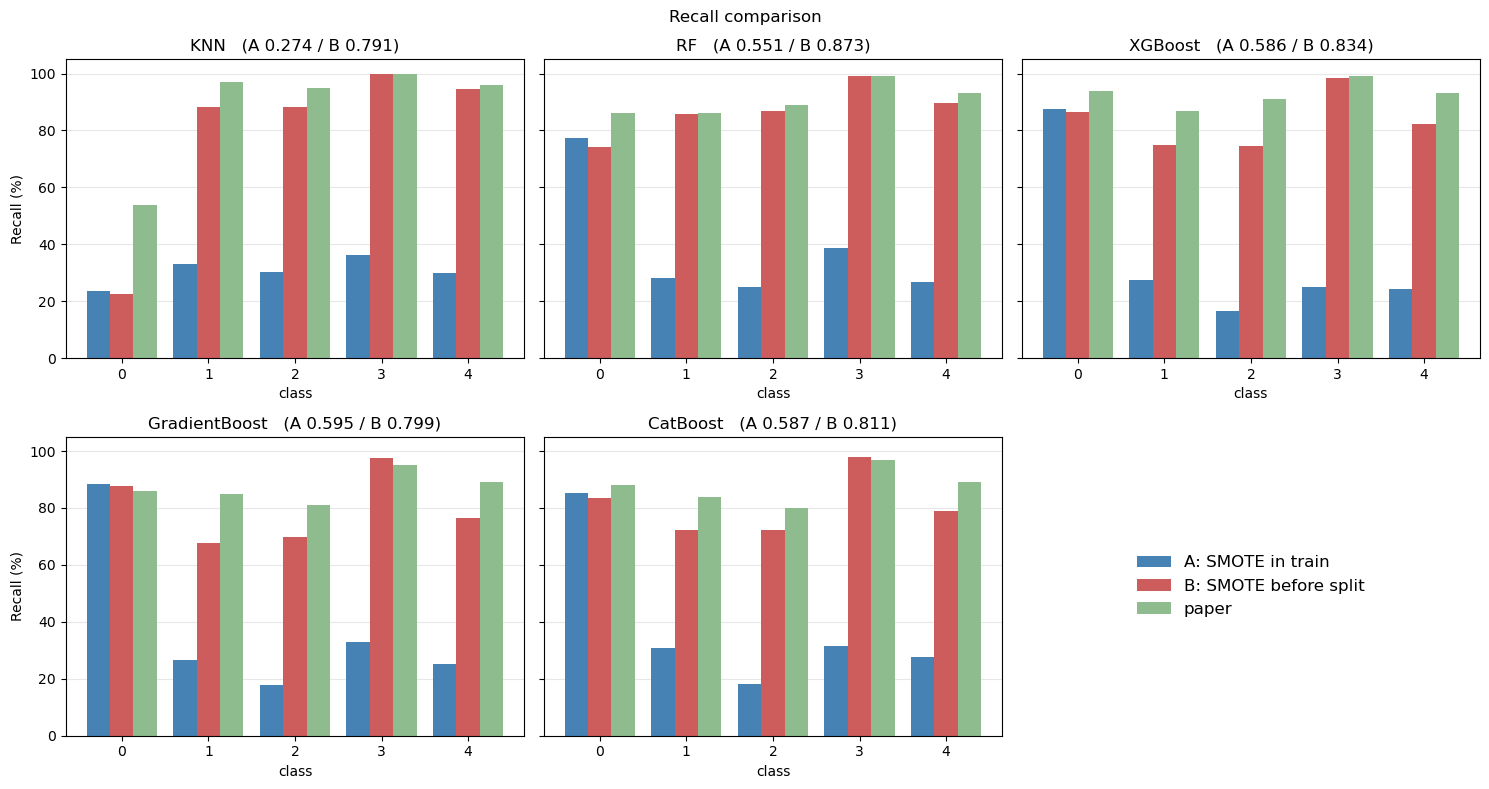
\includegraphics[width=0.9\textwidth]{figures/part1/ablation_recall.png}
\end{figure}

\begin{figure}[H]
    \caption{Comparison on class–wise F1 for each model.}
    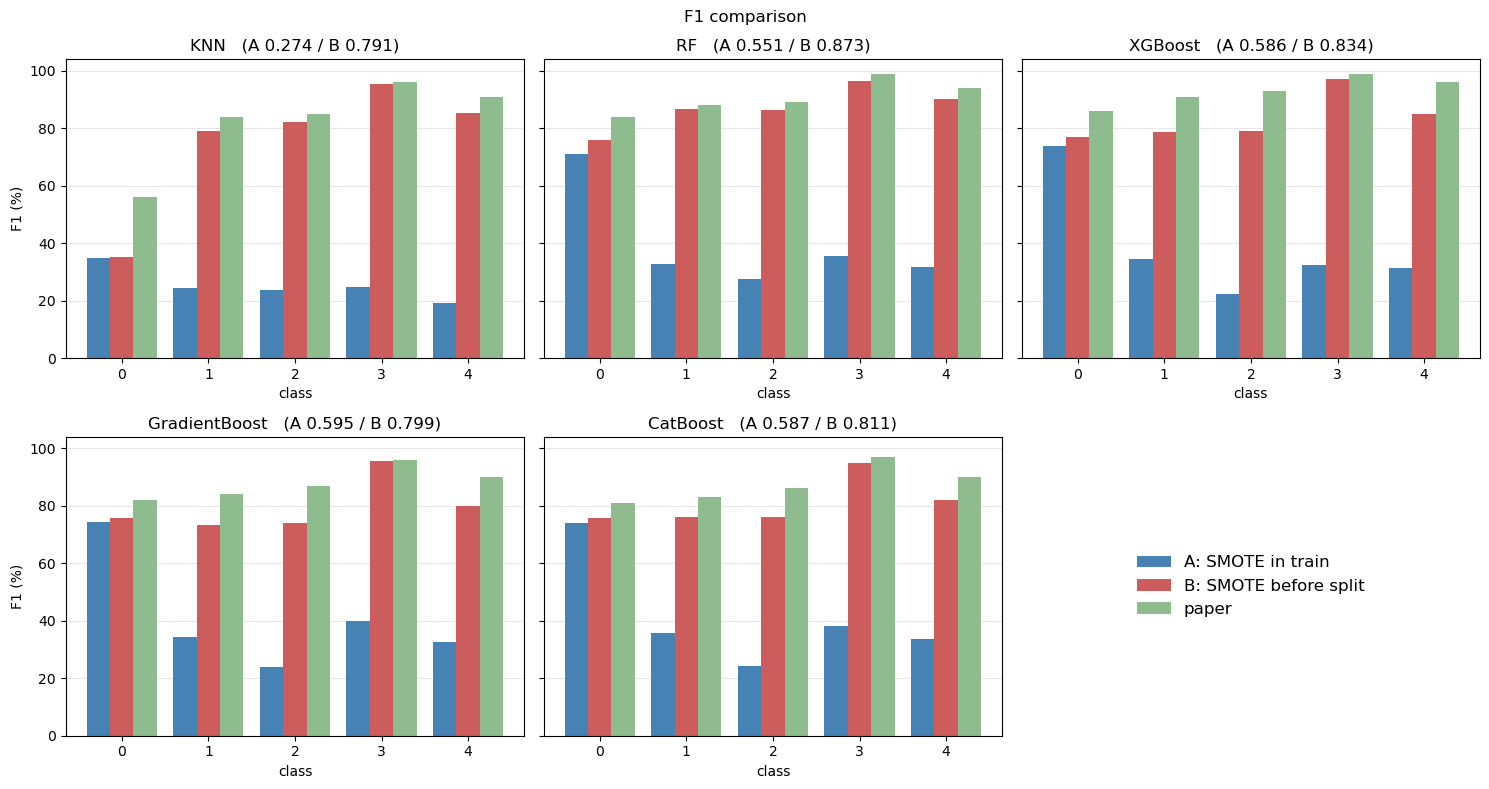
\includegraphics[width=0.9\textwidth]{figures/part1/ablation_f1.png}
\end{figure}

The above–presented bar plots are to aid in the investigation of \textbf{Tab. \ref{tab:cv_classwise_ablation}} visually.
Considering the figures and tables below, although there are moderate deviations from the actual results, we further notice the \textbf{Fig. \ref{fig:ablation_confusion}} and \textbf{Fig. \ref{fig:ablation_roc_curve}} share a very similar patterns.
Interestingly, without further evidence, by changing the flattening strategy, $(12 \times 1000) \to (12000,)$, the gap is much narrower. One can test by switching ``timemajor'' to ``leadmajor'' in \texttt{ablation.ipynb}.

\begin{table}[H]
    \centering
    \caption{\textbf{Protocol B} class–wise performance metrics across models.}
    \label{tab:cv_classwise_ablation}

    \begin{subtable}[t]{0.48\textwidth}
        \centering
        \caption{KNN}
        \label{tab:cv_knn_ablation}
        \begin{tabular}{cccc}
            \toprule
            Class & Precision & Recall & F1 Score \\
            \midrule
            NORM (0) & 81.8 & 23.0 & 35.9 \\
            MI   (1) & 73.4 & 90.8 & 81.2 \\
            STTC (2) & 77.3 & 90.6 & 83.4 \\
            HYP  (3) & 92.4 & 99.9 & 96.0 \\
            CD   (4) & 77.5 & 95.2 & 85.4 \\
            \bottomrule
        \end{tabular}
    \end{subtable}
    \hfill
    \begin{subtable}[t]{0.48\textwidth}
        \centering
        \caption{Random Forest}
        \label{tab:cv_rf_ablation}
        \begin{tabular}{cccc}
            \toprule
            Class & Precision & Recall & F1 Score \\
            \midrule
            NORM (0) & 81.3 & 75.4 & 78.2 \\
            MI   (1) & 88.1 & 87.8 & 87.9 \\
            STTC (2) & 86.7 & 88.7 & 87.7 \\
            HYP  (3) & 94.1 & 99.2 & 96.6 \\
            CD   (4) & 91.0 & 90.8 & 90.9 \\
            \bottomrule
        \end{tabular}
    \end{subtable}

    \bigskip

    \begin{subtable}[t]{0.48\textwidth}
        \centering
        \caption{Histogram–based Gradient Boosting}
        \label{tab:cv_gb_ablation}
        \begin{tabular}{cccc}
            \toprule
            Class & Precision & Recall & F1 Score \\
            \midrule
            NORM (0) & 68.5 & 87.5 & 76.8 \\
            MI   (1) & 79.6 & 69.8 & 74.4 \\
            STTC (2) & 79.1 & 70.6 & 74.6 \\
            HYP  (3) & 93.6 & 97.6 & 95.6 \\
            CD   (4) & 84.5 & 77.0 & 80.5 \\
            \bottomrule
        \end{tabular}
    \end{subtable}
    \hfill
    \begin{subtable}[t]{0.48\textwidth}
        \centering
        \caption{AdaBoost}
        \label{tab:cv_ada_ablation}
        \begin{tabular}{cccc}
            \toprule
            Class & Precision & Recall & F1 Score \\
            \midrule
            NORM (0) & 43.4 & 38.6 & 40.6 \\
            MI   (1) & 32.5 & 32.2 & 32.0 \\
            STTC (2) & 31.5 & 32.3 & 31.6 \\
            HYP  (3) & 58.7 & 71.2 & 64.3 \\
            CD   (4) & 37.5 & 32.1 & 34.4 \\
            \bottomrule
        \end{tabular}
    \end{subtable}

    \bigskip

    \begin{subtable}[t]{0.48\textwidth}
        \centering
        \caption{CatBoost}
        \label{tab:cv_cat_ablation}
        \begin{tabular}{cccc}
            \toprule
            Class & Precision & Recall & F1 Score \\
            \midrule
            NORM (0) & 70.4 & 84.6 & 76.9 \\
            MI   (1) & 81.2 & 73.1 & 76.9 \\
            STTC (2) & 80.3 & 73.3 & 76.6 \\
            HYP  (3) & 92.5 & 98.0 & 95.2 \\
            CD   (4) & 86.2 & 79.8 & 82.8 \\
            \bottomrule
        \end{tabular}
    \end{subtable}
    \hfill
    \begin{subtable}[t]{0.48\textwidth}
        \centering
        \caption{XGBoost}
        \label{tab:cv_xgb_ablation}
        \begin{tabular}{cccc}
            \toprule
            Class & Precision & Recall & F1 Score \\
            \midrule
            NORM (0) & 70.9 & 87.2 & 78.2 \\
            MI   (1) & 84.6 & 76.3 & 80.2 \\
            STTC (2) & 84.3 & 76.2 & 80.0 \\
            HYP  (3) & 96.1 & 98.5 & 97.3 \\
            CD   (4) & 88.3 & 83.0 & 85.5 \\
            \bottomrule
        \end{tabular}
    \end{subtable}
\end{table}



\begin{table}[H]
    \centering
    \caption{\textbf{Protocol B} Performance metrics across all models.}
    \label{tab:single_model_wise_ablation}
    \begin{tabular}{ccccccc}
        \toprule
        Metrics & \texttt{XGBoost} & \texttt{RF} & \texttt{CatBoost} & \texttt{AdaBoost} & \texttt{GBoost} & \texttt{KNN} \\
        \midrule
        Precision & 84.8 & 88.2 & 82.1 & 40.7 & 81.1 & 80.5 \\
        Recall & 84.2 & 88.4 & 81.8 & 41.3 & 80.5 & 79.9 \\
        F1 Score & 84.3 & 88.3 & 81.7 & 40.6 & 80.4 & 76.4 \\
        Accuracy & $84.2$ & $88.4$ & $81.8$ & $41.3$ & $80.5$ & $79.9$ \\
        \bottomrule
    \end{tabular}
\end{table}

\begin{figure}[H]
    \centering
    \caption{\textbf{Protocol A} Confusion matrices of all classifiers.}
    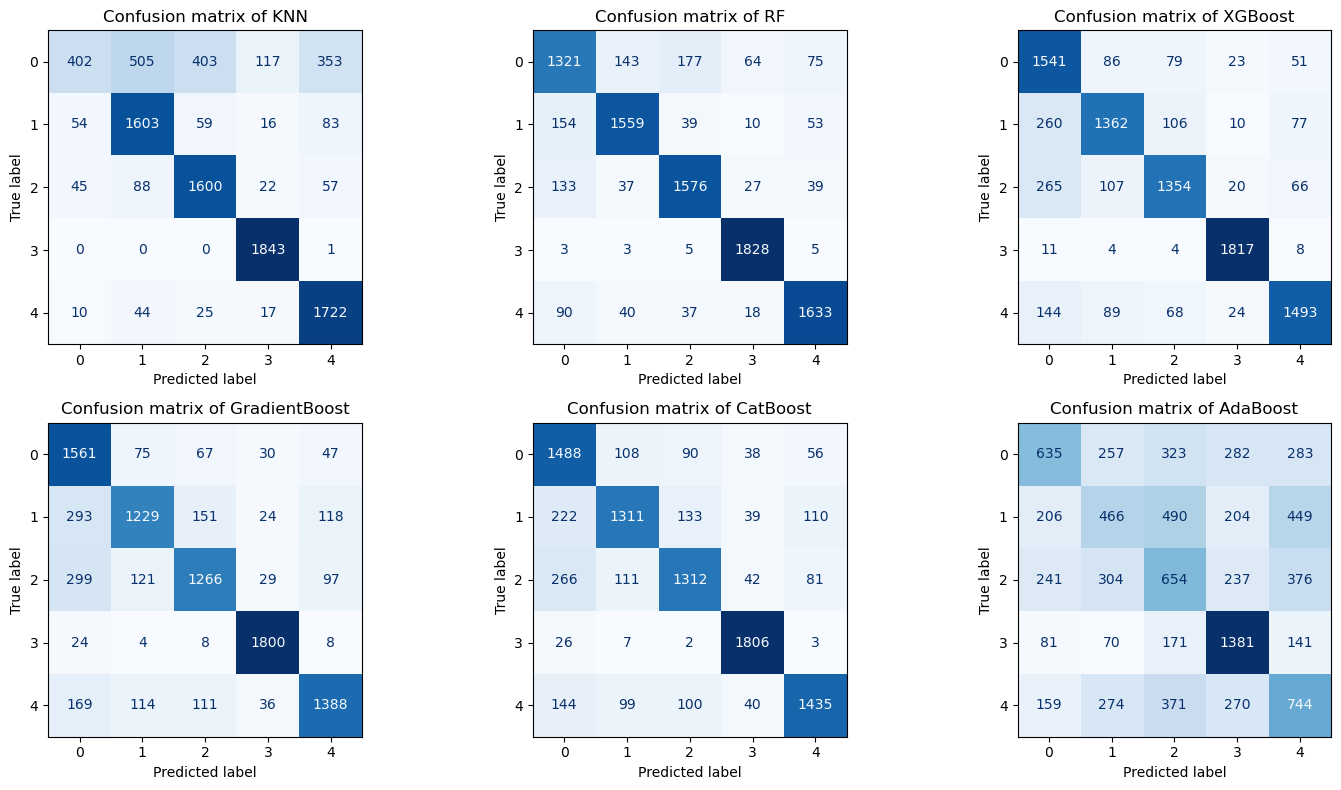
\includegraphics[width=\textwidth]{figures/part1/ablation_confusion.png}
    \label{fig:ablation_confusion}
\end{figure}

\begin{figure}[H]
    \centering
    \caption{\textbf{Protocol A} ROC–AUC curves and scores across classifiers.}
    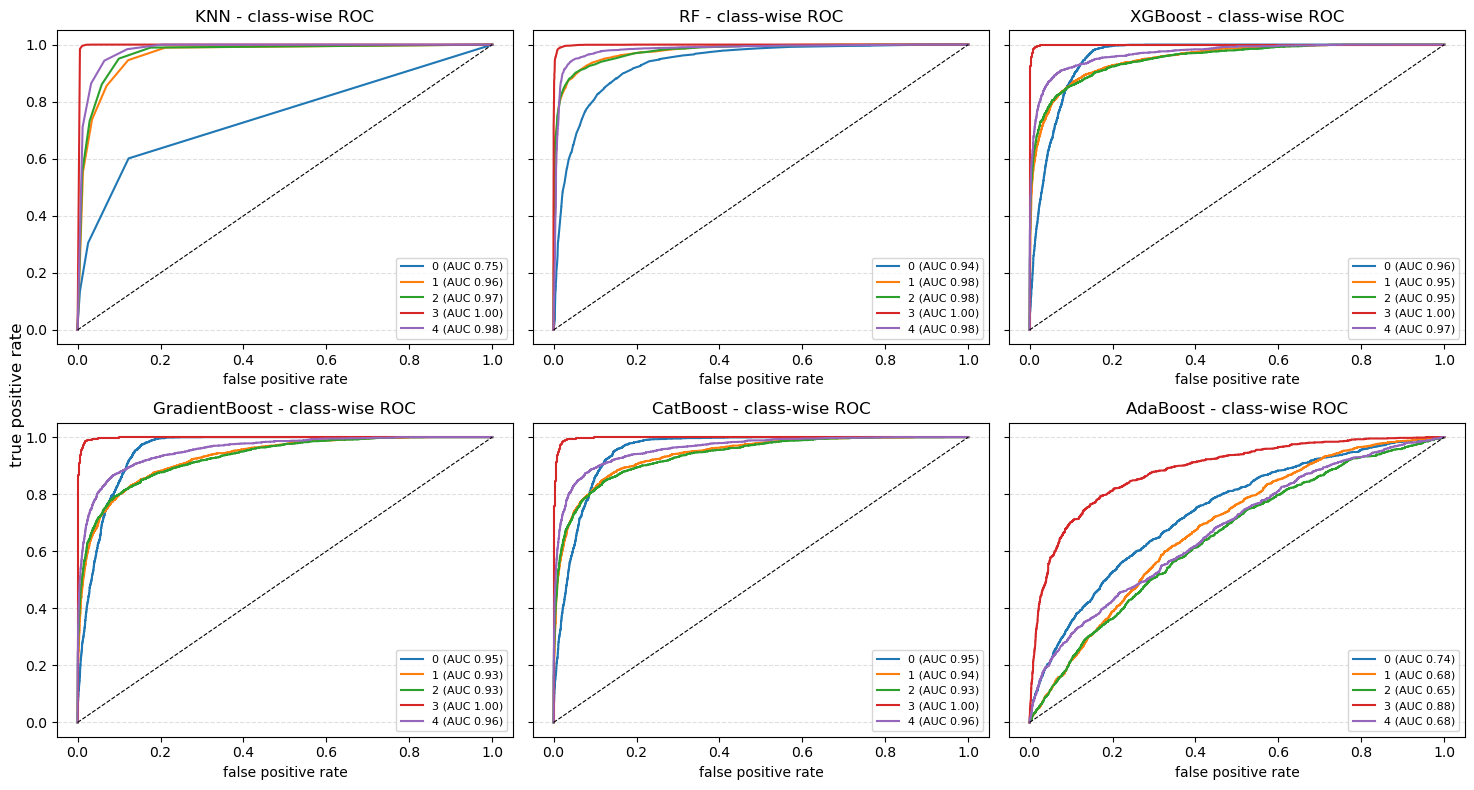
\includegraphics[width=\textwidth]{figures/part1/ablation_roc_curve.png}
    \label{fig:ablation_roc_curve}
\end{figure}

\paragraph{Findings.}
Performing scaling and \texttt{SMOTE} before partitioning takes the ensembles most of the way to the published level.
As the flattening is unchanged from \textbf{Sec. \ref{sec:part_1_method}}, the $39.9$–$49.1$ F1 points the four ensembles gain over \textbf{Tab. \ref{tab:single_model_wise}} are attributable to this leakage alone; \texttt{RF}, for instance, rises from $39.2$ to $88.3$.
The published figures are nevertheless not fully recovered.
All $20$ class–wise F1 scores of \texttt{RF}, \texttt{XGBoost}, \texttt{GBoost} and \texttt{CatBoost} in \textbf{Tab. \ref{tab:cv_classwise_ablation}} fall below the paper's per–class tables \cite{sinha2023dasmcc}, by $0.1$–$13.0$ points, the largest shortfall being STTC under \texttt{XGBoost} ($80.0$ against $93$).
\texttt{RF} comes closest, within $5.8$ points on every class, and replaces \texttt{XGBoost} as the best model; the four ensembles span $80.5$–$88.4\%$ accuracy, against $88.0$–$93.0\%$ in their Table 12.
For the boosted models, NORM precision ($68.5$–$70.9$) lies well below its recall ($84.6$–$87.5$), since \textbf{Fig. \ref{fig:ablation_confusion}} shows minority records absorbed into NORM, e.g. $260$ MI and $265$ STTC records under \texttt{XGBoost}.
\texttt{KNN} still fails on NORM, with F1 $35.9$ against the published $56$, classifying only $402$ of $1{,}780$ NORM records correctly.

Three observations confirm that the leakage reproduces the paper's protocol.
First, recall equals accuracy for all six models in \textbf{Tab. \ref{tab:single_model_wise_ablation}}, which holds only when every class has equal support.
Second, \textbf{Fig. \ref{fig:ablation_confusion}} contains $9{,}069$ test samples spread almost evenly across the classes ($1{,}780$–$1{,}844$ each), mirroring the $9{,}083$ in the paper, whereas a leakage–free $80/20$ split yields $3{,}249$.
Third, HYP, only $3.8\%$ of a leakage–free test split, becomes the easiest class: its F1 is $95.2$–$97.3$ for every model except \texttt{AdaBoost}, and its AUC in \textbf{Fig. \ref{fig:ablation_roc_curve}} reaches $1.00$ for those five models, matching the paper's $1.00$.
